% BAC 2025 D - Exercice 2
% Plan complexe - Points A, B, C

\documentclass[border=5pt]{standalone}
\usepackage{tikz}
\usepackage{amsmath}
\usepackage{amssymb}

\begin{document}

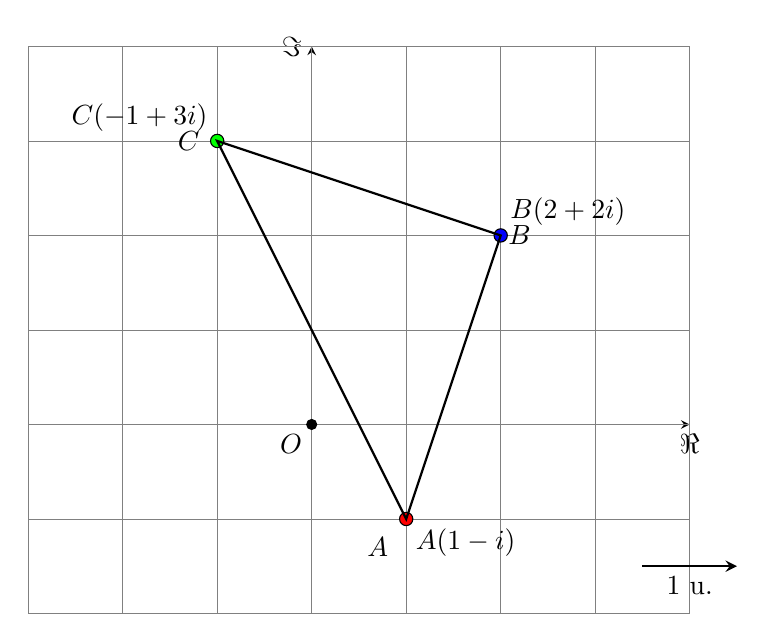
\begin{tikzpicture}[scale=1.2, >=stealth]

% Axes
\draw[->] (-3,0) -- (4,0) node[below] {$\Re$};
\draw[->] (0,-2) -- (0,4) node[left] {$\Im$};

% Grid (optional)
\draw[help lines] (-3,-2) grid (4,4);

% Point A: z_A = 1 - i
\coordinate (A) at (1,-1);
\draw[fill=red] (A) circle (2pt) node[below right] {$A(1-i)$};

% Point B: z_B = 2 + 2i
\coordinate (B) at (2,2);
\draw[fill=blue] (B) circle (2pt) node[above right] {$B(2+2i)$};

% Point C: z_C = -1 + 3i
\coordinate (C) at (-1,3);
\draw[fill=green] (C) circle (2pt) node[above left] {$C(-1+3i)$};

% Triangle ABC
\draw[thick] (A) -- (B) -- (C) -- cycle;

% Labels for vertices
\node at (0.7,-1.3) {$A$};
\node at (2.2,2) {$B$};
\node at (-1.3,3) {$C$};

% Origin O
\draw[fill=black] (0,0) circle (1.5pt) node[below left] {$O$};

% Scale indicator
\draw[->, thick] (3.5,-1.5) -- (4.5,-1.5) node[midway, below] {1 u.};

\end{tikzpicture}

\end{document}